\chapter{Nevronske mreže}

V tem poglavju bomo podrobneje predstavili naprej usmerjene (angl.\ feedforward) umetne nevronske mreže, natančneje večnivojske perceptrone (angl.\ multilayer perceptron). Zaradi boljše berljivosti bomo v nadaljevanju uporabljali zgolj izraz nevronska mreža. Najprej bomo predstavili osnovne koncepte, nato podali matematični model ter opisali algoritem vzvratnega razširjanja napake.

%%%%%%%%%%%%%%%%%%%%%%%%%%%%%%%%%%%%%%%%%%%%%%%%%%%%%%%%%%%%%%%%%%%%%%%%%%%%%%%%%%%%%%%%%%%%%

\section{Osnovni koncepti}

Umetna nevronska mreža je matematični model, ki posnema delovanje človeških možganov. Predstavljamo si jo lahko kot usmerjen acikličen graf, kjer so vozlišča oziroma nevroni urejeni v zaporedne sloje. Povezave med njimi so utežene in potekajo izključno med nevroni sosednjih slojev, v smeri od prvega (vhodnega) sloja proti zadnjemu (izhodnemu) sloju. Sloje običajno razdelimo na tri tipe:
\begin{itemize}
  \item \textbf{Vhodni sloj} je prvi sloj, ki sprejme vhodne podatke in jih brez sprememb posreduje skritemu sloju. Število nevronov v tem sloju ustreza dimenziji vhodne množice.
  \item \textbf{Skriti sloji} se nahajajo med vhodnim in izhodnim slojem ter so odgovorni za večino obdelave podatkov. Njihovo število in velikost se lahko poljubno prilagajata glede na kompleksnost problema.
  \item \textbf{Izhodni sloj} je zadnji sloj in vrne končni rezultat, ki predstavlja napoved mreže. Število nevronov v tem sloju je odvisno od vrste problema – pri regresiji je to običajno en nevron, pri klasifikaciji pa en nevron za vsak razred. 
\end{itemize}

\begin{figure}[H]
  \centering
  % LAYERS IN NEURAL NETWORK
\begin{tikzpicture}[scale=1.25,x=2.2cm,y=1.4cm]

  \message{^^Layers in Neural network}
  \readlist\Nnod{4,5,5,5,3} % array of number of nodes per layer
  \readlist\Nstr{n,m,m,m,k} % array of string number of nodes per layer
  % \readlist\Cstr{\strut x,a^{(\prev)},a^{(\prev)},a^{(\prev)},y} % array of coefficient symbol per layer
  \def\yshift{0.5} % shift last node for dots
  
  \message{^^Drawing Layers}
  \foreachitem \N \in \Nnod{ % loop over layers
    \def\lay{\Ncnt} % alias of index of current layer
    \pgfmathsetmacro\prev{int(\Ncnt-1)} % number of previous layer
    \message{\lay,}
    \foreach \i [evaluate={\c=int(\i==\N); \y=\N/2-\i-\c*\yshift;
                 \index=(\i<\N?int(\i):"\Nstr[\lay]");
                 \x=\lay; \n=\nstyle;}] in {1,...,\N}{ % loop over nodes
      % NODES
      \node[node \n] (N\lay-\i) at (\x,\y) {}; % {$\Cstr[\lay]_{\index}$};
      
      % CONNECTIONS
      \ifnum\lay>1 % connect to previous layer
        \foreach \j in {1,...,\Nnod[\prev]}{ % loop over nodes in previous layer
          \draw[connect arrow, gray] (N\prev-\j) -- (N\lay-\i); % connect arrows directly
        }
      \fi % else: nothing to connect first layer
      
    }
    \path (N\lay-\N) --++ (0,1+\yshift) node[midway,scale=1.5] {$\vdots$};
  }
  
  % RECTANGLE
  \node[
    draw=myblue!40,
    fill=myblue,
    fill opacity=0.02,
    rounded corners=2,
    inner sep=10pt,
    fit=(N2-1)(N4-5)
  ] {};

  % LABELS
  \node[above=5,align=center,softorange!60!black] at (N1-1.90) {vhodni\\[-0.2em]sloj};
  \node[above=10,align=center,myblue!60!black] at (N3-1.90) {skriti sloji};
  \node[above=5,align=center,myred!60!black] at (N\Nnodlen-1.90) {izhodni\\[-0.2em]sloj};
  
\end{tikzpicture}

  \caption{Sloji v nevronski mreži}~\label{fig:nn-layers}
\end{figure}

Izhodno vrednost nevrona imenujemo aktivacija. Vsak nevron sprejme aktivacije nevronov iz prejšnjega sloja, oziroma vhodne podatke v primeru prvega sloja. Iz teh vrednosti izračuna uteženo vsoto, nato pa rezultat preslika s t.\  i.\ aktivacijsko funkcijo. Aktivacijska funkcija je praviloma nelinearna, kar zagotavlja nelinearnost modela.
Da bi utežena vsota lahko vsebovala konstantni člen, vsakemu sloju razen izhodnega dodamo po en nevron s konstantno aktivacijo ena.

\begin{figure}[H]
  \centering
  \tikzset{
  connect arrow/.style={->, draw=gray}
}

% LAYERS IN NEURAL NETWORK
\begin{tikzpicture}[scale=1.25,x=2.2cm,y=1.4cm]

  \message{^^Layers in Neural network}
  \readlist\Nnod{4,5,5,5,3} % array of number of nodes per layer
  \readlist\Nstr{n,m,m,m,k} % array of string number of nodes per layer
  % \readlist\Cstr{\strut x,a^{(\prev)},a^{(\prev)},a^{(\prev)},y} % array of coefficient symbol per layer
  \def\yshift{0.5} % shift last node for dots
  
  \message{^^Drawing Layers}
  \foreachitem \N \in \Nnod { % loop over layers
    \def\lay{\Ncnt} % current layer index
    \pgfmathsetmacro\prev{int(\Ncnt - 1)} % previous layer index
    \message{\lay,}

    % Number of total nodes in this layer including bias if not last
    \ifnum\lay<\Nnodlen
      \pgfmathsetmacro\Nwithbias{\N + 1}
      \def\firstIndex{0}
    \else
      \pgfmathsetmacro\Nwithbias{\N}
      \def\firstIndex{1}
    \fi

    % All neurons in layer: bias (index 0) + regular (1..N)
    \foreach \i [evaluate={
        \c=int(\i==\N);
        \y=\N/2-\i-\c*\yshift;
        \x=\lay; \n=\nstyle;
      }] in {\firstIndex,...,\N} {

      % \node[node \n] (N\lay-\i) at (\x,\y) {};

      \ifnum\i=0
        % \node[circle, draw=teal!60!black, fill=teal!20, minimum size=8pt, inner sep=2pt] (N\lay-\i) at (\x,\y) {};
        \node[node bias] (N\lay-\i) at (\x,\y) {+1};
      \else
        \node[node \n] (N\lay-\i) at (\x,\y) {};
      \fi

      % Only connect if NOT bias node
      \ifnum\i>0
        \ifnum\lay>1
          \ifnum\prev<\Nnodlen
            \foreach \j in {0,...,\Nnod[\prev]} {
              \draw[connect arrow] (N\prev-\j) -- (N\lay-\i);
            }
          \else
            \foreach \j in {1,...,\Nnod[\prev]} {
              \draw[connect arrow] (N\prev-\j) -- (N\lay-\i);
            }
          \fi
        \fi
      \fi
    }

    % Dots
    \path (N\lay-\N) --++ (0,1+\yshift) node[midway,scale=1.5] {$\vdots$};
  }
  
  % RECTANGLE
  % \node[
  %   draw=myblue!40,
  %   fill=myblue,
  %   fill opacity=0.02,
  %   rounded corners=2,
  %   inner sep=10pt,
  %   fit=(N2-1)(N4-5)
  % ] {};

  % LABELS
  % \node[above=5,align=center,softorange!60!black] at (N1-1.90) {vhodni\\[-0.2em]sloj};
  % \node[above=10,align=center,myblue!60!black] at (N3-1.90) {skriti sloji};
  % \node[above=5,align=center,myred!60!black] at (N\Nnodlen-1.90) {izhodni\\[-0.2em]sloj};
  
\end{tikzpicture}

  \caption{Nevron s konstantno aktivacijo}~\label{fig:nn-bias}
\end{figure}

%%%%%%%%%%%%%%%%%%%%%%%%%%%%%%%%%%%%%%%%%%%%%%%%%%%%%%%%%%%%%%%%%%%%%%%%%%%%%%%%%%%%%%%%%%%%%

\section{Matematični model}

V nadaljevanju bomo definirali notacijo, ki je pogosto uporabljena v strokovni literaturi s področja umetne inteligence, na primer v~\cite{Hastie2009}. Takšna notacija omogoča dosledno in formalno predstavitev nevronskih mrež.

Naj bo nevronska mreža sestavljena iz $k+1$ slojev, označenih z $L^{(0)}, L^{(1)}, \dots, L^{(k)}$, kjer je $L^{(0)}$ vhodni sloj, $L^{(k)}$ pa izhodni sloj. Vsak sloj $L^{(i)}$ vsebuje $N^{(i)}$ nevronov, za $i = 0, \dots, k$.

Vhod v mrežo predstavimo z vektorjem $x \in \mathbb{R}^{N^{(0)}}$, ki vsebuje $N^{(0)}$ komponent in služi kot začetna aktivacija v vhodnem sloju.

Za vsak sloj $L^{(i)}$ definiramo:

\begin{itemize}
  \item $a^{(i)}$ aktivacijska funkcija v sloju $L^{(i)}$.
  
  \item $h^{(i)} = \left(h^{(i)}_1, h^{(i)}_2, \dots, h^{(i)}_{N^{(i)}}\right)$ je vektor aktivacij v sloju $L^{(i)}$. Za vhodni sloj velja $h^{(0)} = x$.
  
  \item $z^{(i)} = \left(z^{(i)}_1, z^{(i)}_2, \dots, z^{(i)}_{N^{(i)}}\right)$ je vektor uteženih vsot v sloju $L^{(i)}$, pri čemer vsaka komponenta predstavlja vsoto uteženih vhodov za posamezen nevron:
  \[
    z^{(i)}_j = \sum_{\ell=1}^{N^{(i-1)}} w^{(i)}_{j\ell} h^{(i-1)}_\ell + b^{(i)}_j, \quad \text{za } j = 1, \dots, N^{(i)}.
  \]

  \item $W^{(i)}$ je matrika uteži dimenzije $N^{(i)} \times N^{(i-1)}$, ki povezuje sloj $L^{(i-1)}$ s slojem $L^{(i)}$. Ima naslednjo obliko:
  \[
    W^{(i)} = \begin{bmatrix}
      w^{(i)}_{1,1} & w^{(i)}_{1,2} & \cdots & w^{(i)}_{1,N^{(i-1)}} \\
      w^{(i)}_{2,1} & w^{(i)}_{2,2} & \cdots & w^{(i)}_{2,N^{(i-1)}} \\
      \vdots       & \vdots       & \ddots & \vdots               \\
      w^{(i)}_{N^{(i)},1} & w^{(i)}_{N^{(i)},2} & \cdots & w^{(i)}_{N^{(i)},N^{(i-1)}}
    \end{bmatrix}
  \]

  \item $b^{(i)} = \left(b^{(i)}_1, b^{(i)}_2, \dots, b^{(i)}_{N^{(i)}}\right)$ je vektor uteži nevronov s konstantno aktivacijo (angl.\ bias) za sloj $L^{(i)}$.
\end{itemize}

Aktivacije v sloju $L^{(i)}$ izračunamo s pomočjo aktivacijske funkcije $a^{(i)}$, ki se uporablja po komponentah:
  \[
    h^{(i)}_j = a^{(i)}\left(z^{(i)}_j\right), \quad \text{za } j = 1, \dots, N^{(i)}.
  \]

Postopek se iterativno izvede za sloje $i = 1, \dots, k$, pri čemer vektor $h^{(k)}$ predstavlja izhod mreže.

\begin{figure}[H]
  \centering
  % NEURAL NETWORK activation with bias
\begin{tikzpicture}[x=2.7cm,y=1.6cm]

  \message{^^JNeural network activation}
  \def\NI{5} % number of regular nodes in input layer
  \def\NO{4} % number of nodes in output layer
  \def\yshift{0.4} % shift last node for dots

  % Total number of input nodes including bias
  \pgfmathsetmacro{\NItotal}{\NI + 1}

  % INPUT LAYER: Bias is node 0, rest from 1 to \NI
  \foreach \i [evaluate={
      \c=int(\i==\NI);
      \y = \NItotal/2 - \i - \c*\yshift;
      \index = (\i==0 ? "b" : (\i==\NI ? "N^0" : int(\i)));
    }] in {0,...,\NI} {
    
    \ifnum\i=0
      % Bias node
      \node[node bias] (NI-\i) at (0,\y) {$1$};
    \else
      % Regular input nodes
      \node[node in,outer sep=0.6] (NI-\i) at (0,\y) {$h_{\index}^{(0)}$};
    \fi
  }

  % OUTPUT LAYER
  \foreach \i [evaluate={\c=int(\i==\NO); \y=\NO/2-\i-\c*\yshift; \index=(\i<\NO?int(\i):"N^1");}]
           in {\NO,...,1} {

    % Highlighted first output neuron
    \ifnum\i=1
      \node[node hidden] (NO-\i) at (1,\y) {$h_{\index}^{(1)}$};
      \foreach \j [evaluate={\index=(\j<\NI?int(\j):"N^0");}] in {0,...,\NI} {
      \draw[connect arrow,white,line width=1.2] (NI-\j) -- (NO-\i);
      \ifnum\j=0
        \draw[connect arrow] (NI-\j) -- (NO-\i)
          node[pos=0.5] {\contour{white}{$b_{1}^{(1)}$}};
      \else
        \draw[connect arrow] (NI-\j) -- (NO-\i)
          node[pos=0.50] {\contour{white}{$w^{(1)}_{1,\index}$}};
      \fi
    }

    \else
      \node[node,blue!20!black!80,draw=myblue!20,fill=myblue!5]
        (NO-\i) at (1,\y) {$h_{\index}^{(1)}$};
      \foreach \j in {0,...,\NI} {
        \draw[connect arrow,gray] (NI-\j) -- (NO-\i);
      }
    \fi
  }

  % DOTS
  \path (NI-\NI) --++ (0,1+\yshift) node[midway,scale=1.2] {$\vdots$};
  \path (NO-\NO) --++ (0,1+\yshift) node[midway,scale=1.2] {$\vdots$};

  % EQUATIONS
  \def\agr#1{{\color{myorange}h_{#1}^{(0)}}}
  \node[below=16,right=11,mydarkblue,scale=0.95] at (NO-1)
    {$\begin{aligned}
       &= \color{mydarkred}a^{(1)}\left( \color{black}
            w^{(1)}_{1,1}\agr{1} + w^{(1)}_{1,2}\agr{2} + \ldots + w^{(1)}_{1,N^0}\agr{n} + b_1^{(1)}
          \color{mydarkred}\right)\\
       &= \color{mydarkred}a^{(1)}\left( \color{black}
            \sum_{i=1}^{n} w^{(1)}_{1,i}\agr{i} + b_1^{(1)}
           \color{mydarkred}\right)= a^{(1)}(z^{(1)})
     \end{aligned}$};
  \node[right,scale=0.9] at (1.3,-1.3)
    {$\begin{aligned}
      {\color{mydarkblue}
      \begin{pmatrix}
        h_{1}^{(1)} \\[0.3em]
        h_{2}^{(1)} \\
        \vdots \\
        h_{N^1}^{(1)}
      \end{pmatrix}}
      &=
      \color{mydarkred}a^{(1)}\left[ \color{black}
      \begin{pmatrix}
        w^{(1)}_{1,1} & w^{(1)}_{1,2} & \ldots & w^{(1)}_{1,N^0} \\
        w^{(1)}_{2,1} & w^{(1)}_{2,2} & \ldots & w^{(1)}_{2,N^0} \\
        \vdots  & \vdots  & \ddots & \vdots  \\
        w^{(1)}_{N^1,1} & w^{(1)}_{N^1,2} & \ldots & w^{(1)}_{N^1,N^0}
      \end{pmatrix}
      {\color{myorange}
      \begin{pmatrix}
        h_{1}^{(0)} \\[0.3em]
        h_{2}^{(0)} \\
        \vdots \\
        h_{N^0}^{(0)}
      \end{pmatrix}}
      +
      \begin{pmatrix}
        b_{1}^{(1)} \\[0.3em]
        b_{2}^{(1)} \\
        \vdots \\
        b_{N^1}^{(1)}
      \end{pmatrix}
      \color{mydarkred}\right]\\[0.5em]
      {\color{mydarkblue}\mathbf{h}^{(1)}}
      &= \color{mydarkred}a^{(1)}\left( \color{black}
           \mathbf{W}^{(1)} {\color{myorange}\mathbf{h}^{(0)}}+\mathbf{b}^{(1)}
         \color{mydarkred}\right)
    \end{aligned}$};

\end{tikzpicture}

  \caption{Aktivacija nevrona v prvem sloju}~\label{fig:nn-activation}
\end{figure}

%%%%%%%%%%%%%%%%%%%%%%%%%%%%%%%%%%%%%%%%%%%%%%%%%%%%%%%%%%%%%%%%%%%%%%%%%%%%%%%%%%%%%%%%%%%%%

\section{Vzvratno razširjanje napake}

Vzrvratno razširjanje napake je metoda za učenje nevronskih mrež. Metoda temelji na minimizaciji funkcije napake z uporabo gradientnega spusta. 

\begin{comment}
Za učinkovito izračun gradientov uteži glede na vrednost funkcije napake uporabimo algoritem \emph{povratnega širjenja napake} (angl.\ \textit{backpropagation}).
\end{comment}

Algoritem temelji na uporabi verižnega pravila (angl.\ \textit{chain rule}) za izračun parcialnih odvodov funkcije napake glede na parametre modela. Proces poteka v dveh fazah:
\begin{enumerate}
  \item \textbf{Propagacija naprej:} za dan vhodni vektor $x$ izračunamo aktivacije vseh slojev $h^{(1)}, h^{(2)}, \dots, h^{(k)}$ in dobimo izhod modela $h^{(k)}$.
  \item \textbf{Propagacija nazaj:} izhod primerjamo s ciljno vrednostjo $y$ in izračunamo napako. Nato postopno računamo gradient funkcije napake $E$ po slojih navzdol, pri čemer za vsak sloj $i$ izračunamo odvod $\frac{\partial E}{\partial W^{(i)}}$ in $\frac{\partial E}{\partial b^{(i)}}$.
\end{enumerate}

Za izračun napake v izhodnem sloju uporabimo izraz:
\[
\delta^{(k)} = \nabla_{h^{(k)}} E \odot \sigma' \left(z^{(k)} \right),
\]
kjer $\odot$ označuje Hadamardov produkt, $E$ je funkcija napake, $\sigma'$ pa odvod aktivacijske funkcije.

Za vse preostale sloje $i = k-1, \dots, 1$ pa napako računamo rekurzivno:
\[
\delta^{(i)} = \left( W^{(i+1)^\top} \delta^{(i+1)} \right) \odot \sigma'\left(z^{(i)}\right).
\]

Posodobitev parametrov nato izvedemo z gradientnim spustom:
\[
W^{(i)} := W^{(i)} - \eta \frac{\partial E}{\partial W^{(i)}}, \qquad
b^{(i)} := b^{(i)} - \eta \frac{\partial E}{\partial b^{(i)}},
\]
kjer je $\eta$ hitrost učenja (angl.\ \textit{learning rate}).

Algoritem povratnega širjenja napake je temeljni gradnik učenja v globokem učenju, saj omogoča učinkovito učenje parametrov tudi v zelo globokih mrežah.



V razdelku bomo opisali algoritem vzratnega razširjanja napake, ki je verjetno eden izmed najbolj študiranih algoritmov učenja nevronskih mrež. Sledili bomo razlagi~\cite{rojas1996backpropagation}.
Učenje v nevronski mreži poteka s prilagajanjem uteži tako, da minimiziramo razlike med dejanskimi izhodnimi vrednostmi in tistimi, ki jih mreža napove. Temu pravimo nadzorovano učenje, kjer imamo podano učno množico podatkov v obliki parov vektorjev vhodnih in izhodnih vrednosti: $\left\{ (x_i, t_i) \mid i = 1, \ldots, p \right\}$ in iz njih lahko izračunamo napako izhodnega sloja:
\begin{equation}
  E = \frac{1}{2} \sum_{i=1}^{p} \|\mathbf{o}_i - \mathbf{t}_i\|^2
\end{equation}
Z $o_{i}$ smo označili izhodne vrednosti ki jih vrne mreža. Ker pa je izhod nevronske mreže pravzaprav funkcija uteži~\ref{eq:eq1}, je tudi $E$ funkcija uteži. Ker Želimo funkcijo napake minimizirati, potrebujemo gradient. Začnemo z zadnjim slojem:
\begin{equation}
  \nabla E = \left( \frac{\partial E}{\partial w^{(k)}_1}, \frac{\partial E}{\partial w^{(k)}_2}, \ldots, \frac{\partial E}{\partial w^{(k)}_m} \right)
\end{equation}
Poskrbeti moramo, še da bo aktivacijska funkcija $a$ odvedljiva, pogosta izbira je sigmoidna funkcija:
\begin{equation}
  \sigma(x) = \frac{1}{1 + e^{-x}}.
\end{equation}
Katere odvod je
\begin{equation}
  \frac{d}{dx}\sigma(x) = \frac{e^{-x}}{\left(1+e^{-x}\right){}^2} = \sigma(x)\left(1 - s(x)\right).
\end{equation}
Sedaj si bo lažje predstavaljati rezultat nevronske mreže in funkcijo napake kot kompozitum velikega števila funkcij in ne več kot rekurzivno funkcijo. Razlog za to je, da bomo lahko pri računanju gradienta uporabili verižno pravilo odvajanja. Uteži nato spreminjamo z metodo gradientnega spusta, ki iterativno zmanjšuje vrednosti uteži v nasprotni smeri vektorja gradienta, dokler ne najde minimuma. Tako se uteži popravijo na zunanjem sloju in nato nadaljujemo s predhodnjim slojem, dokler ne pridemo do začetka. V zadnjem sloju lahko neposredno primerjamo napovedan izhod z dejanskim izhodom, da izračunamo gradient. V skritih slojih pa se gradient izračuna na podlagi gradienta sloja pred njim, od tod izvira ime vzratno razširjanje napake.

\begin{figure}[H]
  \centering
  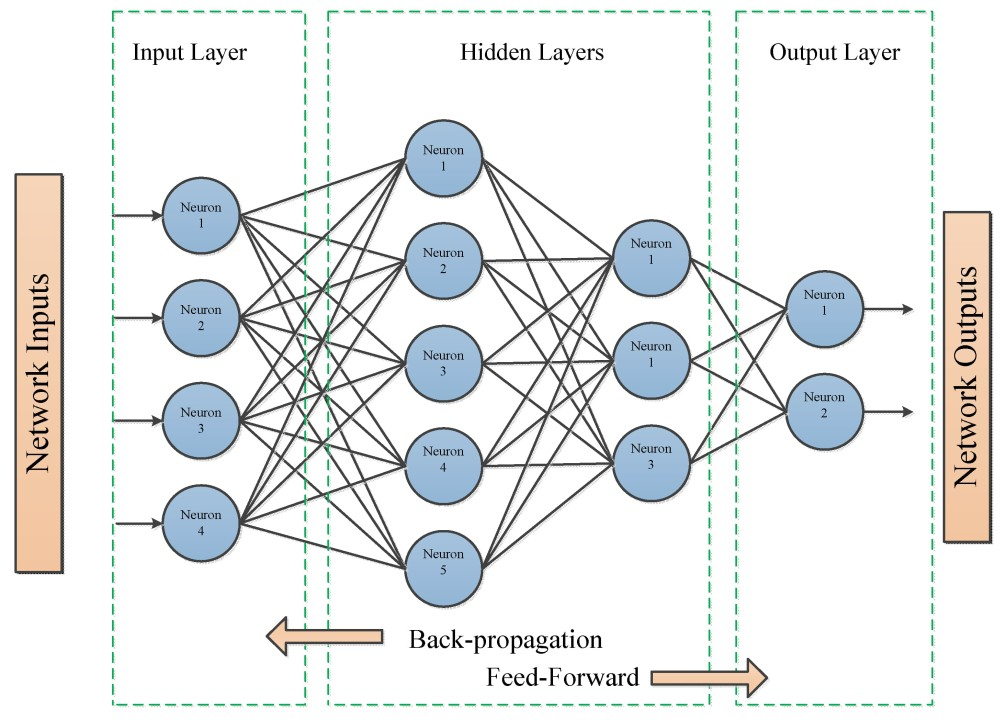
\includegraphics[width=0.7\linewidth]{resources/backpropagation.jpeg}
  \caption{Vzratno razširjanje napake. Vir:~\cite{electronics10212689}}~\label{fig:backprop}
\end{figure}

Od sedaj naprej nas bo samo zanimala evolucija uteži v procesu učenja. Na posameznih slojih bomo opazovali vektorje uteži za vsak nevron, ki jih bomo interpretirali kot točke v visoko dimenzionalnem prostoru. Za vsak sloj $i$ so to  ravno vrstice v matriki uteži $W^{(i)}$. Ker pa si visoko dimenzionalnih prostorov ne moremo predstavljati, se bomo v naslednjem razdelku ukvarjali s tem kako točke preslikati v nižje dimenzionalni prostor s čim manjšo izgubo informacij.

Aktivacije nevronov za sloje $i = 1, 2, \ldots, k$ izračunamo po formuli:
\begin{equation}
  h^{(i)} = a^{(i)}(W^{(i)} \cdot h^{(i - 1)})
\end{equation}

Aktivacijsko funkcijo $a^{(i)}$ definiramo po komponentah. Rezultat nevronske mreže, torej predstavlja zadnji sloj, ki ga lahko s pomočjo zgornje zveze rekurzivno izračunamo:
\begin{equation}
  h^{(k)} = a(W^{(k - 1)} \cdot h^{(k - 1)})
  \label{eq:eq1}
\end{equation}
Ustavitveni pogoj je $h^{(0)}$, ki je vhodni podatek.